\documentclass[11pt,fullpage]{book}
\title{\textbf{~~~~~~~~~~~~~~~}\newline Econometrics book}
\author{Ben Lambert}
\usepackage{natbib}
\usepackage{appendix}
\usepackage{url,times}
\usepackage{graphicx}
\usepackage{epstopdf}
\usepackage{amsmath}
\usepackage[all]{xy}
\usepackage{pxfonts}
\usepackage{colortbl}
\usepackage{color}
\usepackage{subfigure}
\usepackage{gensymb}
\usepackage{ctable}
\usepackage[justification=centering]{caption}[2007/12/23]
\usepackage{longtable}
\usepackage{pstricks-add}
\usepackage{pstricks}
\usepackage{pst-func}
\usepackage{pst-math}
\usepackage{epigraph}



\setlength{\parindent}{0.0in}
\setlength{\parskip}{0.1in}
\maketitle

\begin{document}
\tableofcontents
\part{The basics}
\chapter{How to best use this book}
\chapter{What is econometrics?}

\chapter{Estimators and their purpose}
\section{Chapter mission statement}
After reading this chapter the student will understand the concept of an estimator, and its use in statistics. 

\section{The goal of this chapter}
Statistical inference is the process of drawing conclusions about a population from a sample of observations. Estimators are the tools which statisticians use on samples of data; resulting in estimates of population-wide quantities which can be used to test hypotheses about the wider world. In this chapter the reader will be introduced to the concept of a \textit{sampling distribution}, and how these can be examined to gauge the quality of an estimator. 

\section{What is an estimator, and why should we care?}
We rarely in life have all relevant data available to us before we make a decision. When we decide where to go on holiday, we don't travel to a country, speak first-hand with locals, and taste the local food prior to deciding on a final destination for the family. We don't know perfectly what the weather will be like this afternoon when we get dressed for work. Instead, we extrapolate based on samples of data, and use these as predictive windows into the unknown. Statistical inference is the logical framework that allows us to make reasonable decisions based on our limited access to the facts. 

These limited facts are what is known as a \textit{sample}; by definition a subset of data from a \textit{population} of interest. A population of interest might be the UK 18-30 females. However, it needn't just be applied to people, and could just as easily be defined to be the countries within the EU. All that matters is that the population, as a concept, is a wider entity on which we would like to make well-informed statements. 

\textit{Estimators} are tools that we use on samples that enable us to make \textit{estimates} of quantities within the wider population being investigated. We then use these estimates to test hypotheses about the population, which allow us to better understand the functioning of the world around us.

\begin{figure}
\centering
\scalebox{0.6} 
{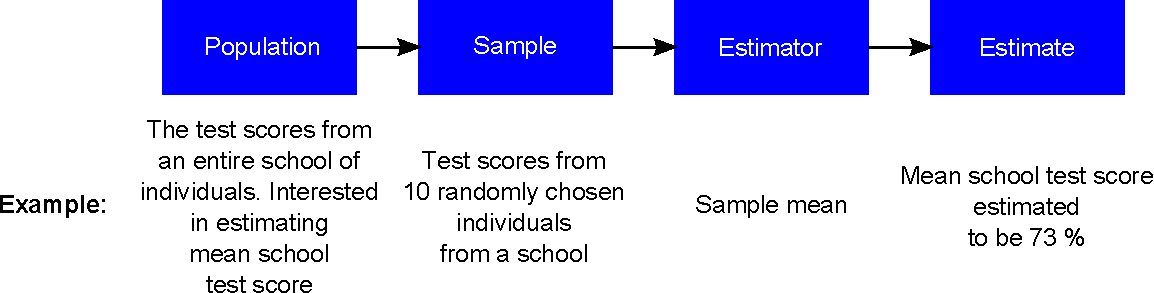
\includegraphics{Estimators_estimatorEstimate.pdf}}
\caption{The estimation process.}\label{fig:Estimators_estimatorEstimate}
\end{figure}

Before we choose an estimator to use, we need to specify a \textit{model} of the population which is proposed as a simplified and tractable representation of real life. Estimators can then be used to estimate components of these models, which when complete, can be deployed to help us explain some key features of a process we observe. Fortunately, statistical inference allows us to test the assumptions on which models are built, as well as interrogate their implications. 

\section{Models}
\epigraph{Essentially, all models are wrong, but some are useful.}{George Box}

Real life in complex. It contains so many, seemingly-independently-moving things, that it can seem difficult/impossible to explain or predict anything effectively. To make life simpler for ourselves, we frequently build \textit{models}. When we are planning how much to budget for electricity this month, we might think that electricity spend in the corresponding month last year might be a reasonable guide. When we are determining how long to spend cramming for an exam, we implicitly have an internal model of the trade off between test score and effort. When we set our alarm for the morning after, we believe that it will roughly take 10 minutes for us to snooze, and another 20 minutes to get showered and ready before leaving the house. These are all examples of models. 

All models are abstractions from reality, which allow us to isolate, and concentrate on what we believe are the important parts of a system of interest. They are necessarily simplifications, and hence are not exactly representative of reality. However, as George Box's quote suggests, they can \textit{sometimes} be useful.

The aforementioned are models which we most likely generate internally, but nonetheless are \textit{implicitly} used to help us make decisions. Often for self-betterment, and to allow interrogation of thought however, we want to \textit{explicitly} describe our models. The language of mathematics provides us with a logical framework with which to adequately describe these abstractions.

Before we talk through examples, it is worth reflecting on the various purposes for building models in the first place. Joshua Epstein in his article 'Why model?' lists amongst others, the following motivations for writing down \textit{explicit} models:

\begin{itemize}
\item Prediction
\item Explanation
\item Guide data collection
\item Discover new questions
\item Bound outcomes to plausible ranges
\item Illuminate uncertainties
\item Challenge the robustness of prevailing theory through perturbations
\item Reveal the apparently simple (complex) to be complex (simple) 
\end{itemize}

There are no doubt other reasons, but I believe that the above covers the majority of rationales.

Imagine we are interested in determining the average test score for a particular standardised exam within the US. We don't have access to test scores for all individuals who take the exam in a specific year however. Instead we might suppose that test scores for individuals in the population are normally distributed about this theoretic mean, $\mu$, with some theoretic variance $\sigma^2$:

\begin{equation}\label{eq:Estimators_normalModelExample}
IQ_i \sim \mathcal{N}\left(\mu,\sigma^2\right)
\end{equation}

In (\ref{eq:Estimators_normalModelExample}), the $i$ subscript on $IQ$ represents the individuals in our population. So if we have a population size of 10,000, $i$ runs from 1 to 10,000. It is important to stress that, whilst in this example, we can suppose that $\mu$ exists, this is not generally the case for quantities of interest in statistics/econometrics. The assumption inherent in the above model is that test scores are normally distributed around this tangible quantity with some theoretic variance. We do not actually believe that test scores are exactly normally distributed\footnote{However, the central limit theorem provides some justification for making this approximation. See section \ref{sec:Estimators_CLT}.}, however to make life easier and more palatable, and thus easier to deal with, we make this approximation. 

Another model which we might choose to state is that there is a linear relationship the number of years of experience and the wage which an individual commands, on average:

\begin{equation}\label{eq:Estimators_modelWageExperienceExample}
wage_i = \alpha + \beta experience_i + \epsilon_i
\end{equation}

In (\ref{eq:Estimators_modelWageExperienceExample}), we have chosen a straight-line\footnote{The model stated in (\ref{eq:Estimators_modelWageExperienceExample}) is, (with the exception of $\epsilon_i$ term), of the form $y = mx + c$, which is taught in high school.} relationship between the experience and wages, apart from a catch-all variable which encapsulates the various other idiosyncratic factors\footnote{Individual attributes.} which might impact the wage an individual obtains. For example, the type of job undertaken, the number of hours worked, or their level of education. We assume here that conditional on the level of experience for individuals, the average effect of these other factors is zero.

A model is only as good as the assumptions on which it rests. It might be that IQ test scores are more variable in the US population, than a normal distribution allows. It could be that there are diminishing returns to experience, meaning that the increment to wage for an extra year of work diminishes, dependent on the stage in the particular individual's career; invalidating the assumption of \textit{linearity}.

Much like models assumptions are necessarily simplifying, and therefore \textit{wrong}. However, there is a spectrum of \textit{wrong}. An assumption is good so long as it captures the essence of reality sufficiently to allow the model to be used as is required. If the assumption is too \textit{wrong}, then the model will cease to be useful, and we are forced to go back and examine its foundations.

\begin{figure}
\centering
\scalebox{0.4} 
{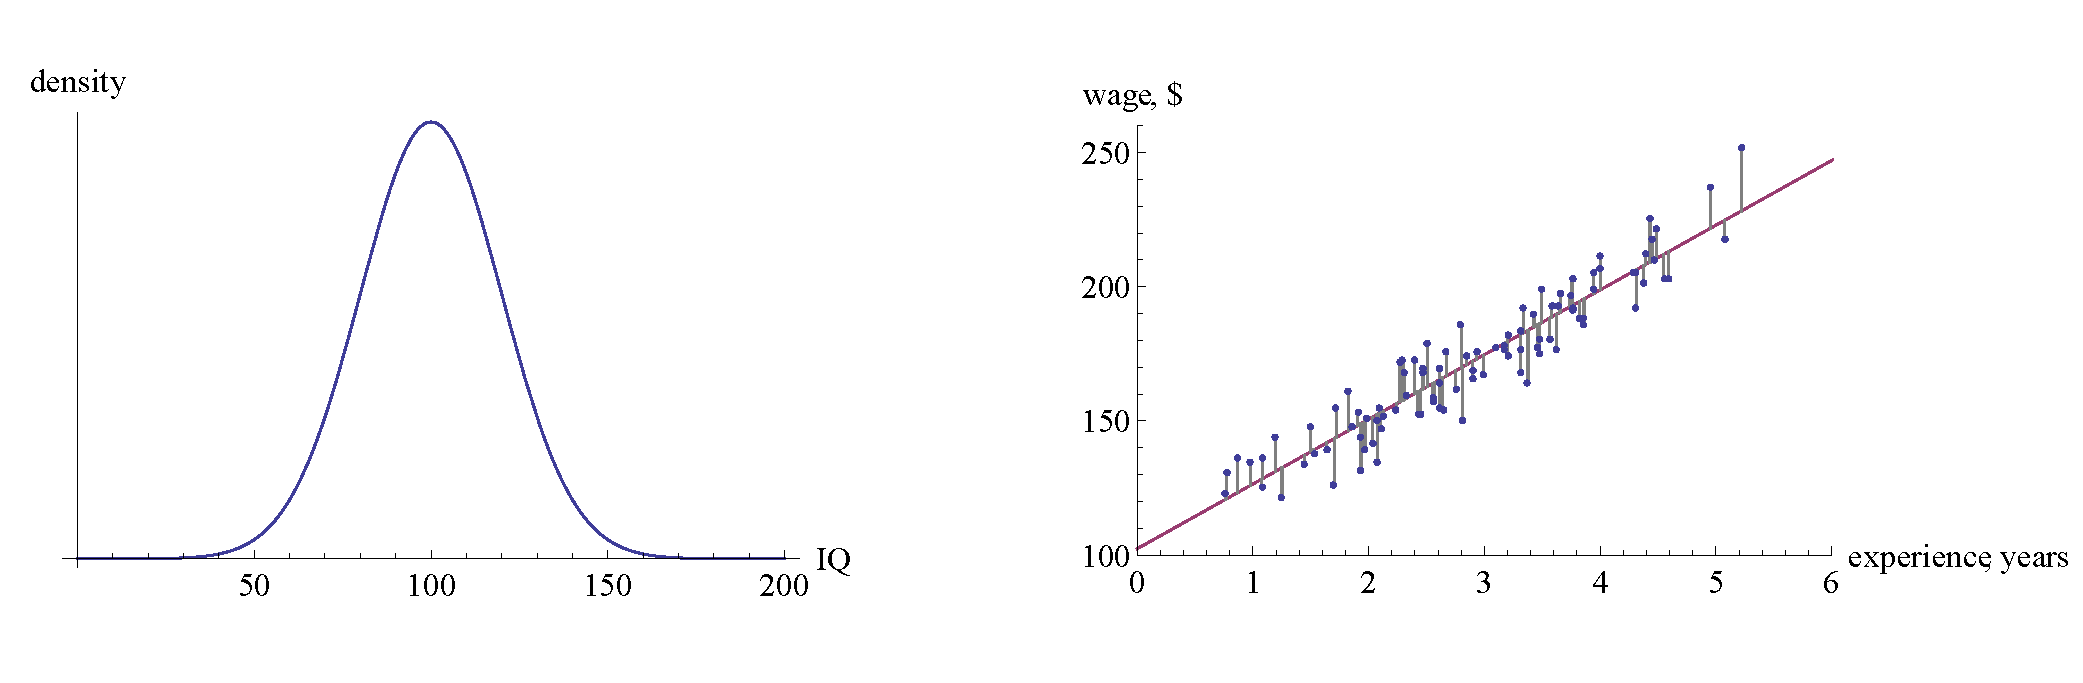
\includegraphics{Estimators_normalIQLinearWage.pdf}}
\caption{Left: the normal model for IQ. Right: the linear model between experience and wages, with the error terms $\epsilon_i$ indicated as vertical deviations from the straight line.}\label{fig:Estimators_normalIQLinearWage}
\end{figure}

\section{Sampling distributions}
\section{Good properties of an estimator}
\section{The central limit theorem}\label{sec:Estimators_CLT}

\part{Cross sectional data: useful and important}
\chapter{When to use Ordinary Least Squares?}
\chapter{How to make conclusions - an introduction to hypothesis testing}
\chapter{How to interpret regression results}
\chapter{Testing the Gauss-Markov assumptions, and what to do if they are violated}
\chapter{Instrumental variables: allowing inference in difficult circumstances}
\chapter{Monte Carlo: How to test the quality of an estimator}

\part{Time series: harder to master, but necessary}
\chapter{Why and how do we need to think about time series differently to cross sectional?}
\chapter{The basic building blocks of time series models: autoregressive and moving averages}
\chapter{Testing for stationarity and what to do with non-stationary data}
\chapter{Cointegration: allowing for realism in time series models}
\chapter{An introduction to models for real processes: partial adjustment and error-correction models}

\part{Panel data: the best of both worlds}
\chapter{The benefits of panel data}
\chapter{Why do we need more estimators? An introduction to First Differences and Fixed Effects}
\chapter{The poor relation: Random Effects}

\part{A simple new paradigm in estimation: Maximum Likelihood}
\chapter{The flaws in the Linear Probability Model}
\chapter{Beautifully simple: An introduction to Maximum Likelihood}
\chapter{Draw conclusions by likelihood: the Wald, the Score and the LM tests}



\bibliographystyle{plain}
\bibliography{Bayes}



\end{document}